% !TeX spellcheck = en_US
%\documentclass[11pt,a4paper]{article}
\documentclass[11pt
  , a4paper
  , article
  , oneside
%  , twoside
%  , draft
]{memoir}

\usepackage{control}
\usepackage[numbers]{natbib}


\begin{document}

\newcommand{\technumber}{
  RAON Control-Document Series\\
  Revision : v1.0,   Release : 2014-12-24 fixed date}
\title{\textbf{EPICS IOC를 위한 EPICS Records 사용법 및 그 개발 방법}}

\author{이상일\thanks{silee7103@ibs.re.kr},이정한\thanks{jhlee@ibs.re.kr}, 손창욱\thanks{cwson@ibs.re.kr},박미정\thanks{mijoy0909@ibs.re.kr} \\

  Rare Isotope Science Project\\
  Institute for Basic Science, Daejeon, South Korea
}
\date{\today}

\renewcommand{\maketitlehooka}{\begin{flushright}\textsf{\technumber}\end{flushright}}
%\renewcommand{\maketitlehookb}{\centering\textsf{\subtitle}}
%\renewcommand{\maketitlehookc}{C}
%\renewcommand{\maketitlehookd}{D}

\maketitle

\begin{abstract}
RAON accelerator는 대형 실험 장치로 많은 실험 장치들과 부대시설 장치로 구성되어 운영된다. 이러한 많은 실험 장치들을 제어하기 위한 제어 시스템들은 넓은 범위로 분산되어 구성되어 있으며 이러한 분산 환경에서의 많은 제어시스템들을 전체의 하나의 제어시스템으로 운영하기 위하여 RAON control system은 EPICS software framework을 사용한다. 본 문서는 EPICS 연계 시스템 인터페이스 개발자가 IOC를 개발하기 위하여 사용하는 EPICS record들에 대한 개발 가이드 레퍼런스를 제공하기 위함이다.
\end{abstract}

RAON accelerator에서 각 로컬 제어 시스템과 EPICS framework간의 integration을 위하여 가장 핵심이 되는 부분은 EPICS IOC 개발이다. 그만큼 EPICS의 여러 모듈 중에서 IOC는 그 핵심 모듈이라고 할 수 있다. IOC 모듈에서도 EPICS DB 생성을 위한 record의 사용 및 그 개발 방법은 제어 디바이스와 EPICS framework간의 인터페이스의 핵심이라 할 수 있다. 본 문서는 EPICS base에서 기본적으로 제공되는 records들에 대한 설명과 그 사용 예제를 통하여 IOC 설계 및 개발자들이 참고할 수 있는 가이드를 제시하려 함이며, 또한 base외에 추가적으로 개발된 IOC record의 개발 내용 및 사용 예제를 통하여 IOC record 개발을 체계성 및 일관성을 유지하여 향 후 체계적인 RAON control system software 형상관리에 도움을 주기위한 문서로 사용하기 위함이다.

\clearpage


\chapter{ai, }

\chapter{rdbpostgreSQL}

rdbpostgreSQL record의 개발 목적은 아래와 같다.
\begin{itemize}
	\item EPICS IOC의 값을 DBMS에서 제공하는 풍부한 연산 알고리즘 활용하여 계산
	\item EPICS로 구성된 가속기 operation parameters 들을 자동으로 Database화 하여 관리
	\item 향 후 가속기 Alarm 시스템과 통신사의 SMS DB와 연계하여 해당 운전자 그룹에 자동 Alarm Message 전송
\end{itemize}

\chapter{rdbmySQL}
SRF Test Facility에서 RMS(Radiation Monitoring System)는 radiation 관련 모니터링 데이터를 MySQL 데이터베이스에 저장한다. 이 저장된 radiation 정보를 통합 operation 관점에서 상시 모니터링 되어야 하므로 MySQL의 데이터베이스와 EPICS간의 인터페이스를 위한 record이다.

rdbmySQL record의 개발 목적은 아래와 같다.
\begin{itemize}
	\item MySQL 데이터베이스와의 interface.
	\item EPICS로 구성된 가속기 operation parameters 들을 자동으로 Database화 하여 관리
\end{itemize}

그림 \ref{fig:rms_epics_db}는 rdbmySQL record를 이용하여 RMS t\_values 테이블과 인터페이스하기 위하여 EPICS db를 구성하는 예를 보여준다.

\begin{figure}[h!]
	\centering
	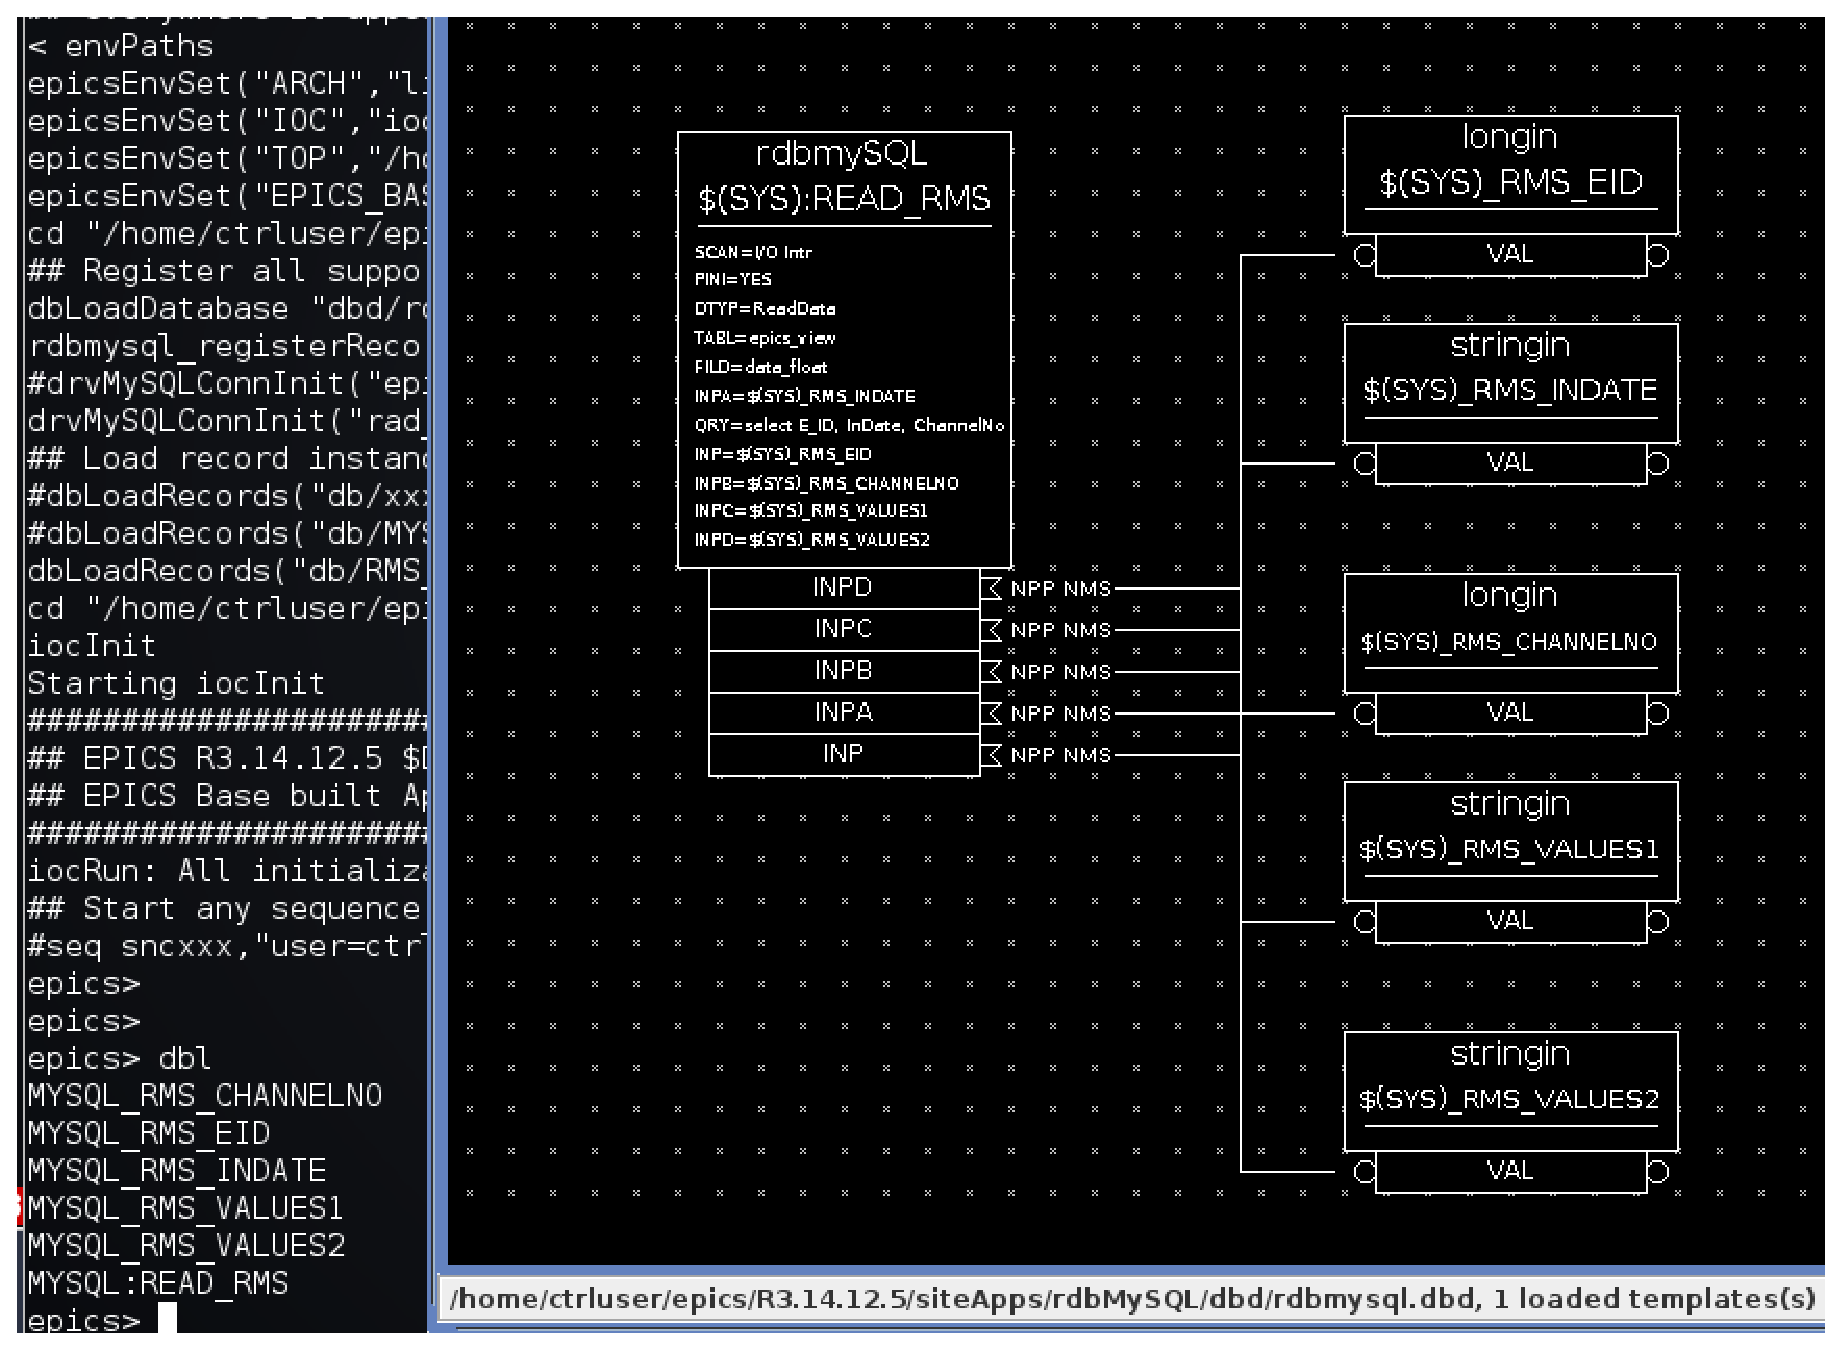
\includegraphics[width=1\textwidth]{./images/rms_epics_db.eps}
	\caption{RMS MySQL 인터페이스를 위한 EPICS DB설정}
	\label{fig:rms_epics_db}
\end{figure}

\begin{figure}[h!]
	\centering
	\includegraphics[width=1\textwidth]{./images/rms_epics_view_trigger.eps}
	\caption{MySQL 트리거링을 이용한 RMS View Table}
	\label{fig:rms_epics_view_trigger}
\end{figure}

\clearpage

\chapter{ifstat}



\begin{itemize}
	\item VxWorks 버전: VxWorks 6.9 (이전 VxWorks 5.5 이하)
	\item IDE 환경 버전: Workbench 3.3 (이전 Tornado 2.2 )
\end{itemize}

Linux에서 Workbench 3.3을 설치하면 기본 설치 디렉토리 경로는 "/opt/WindRiver/" 되며, 이것과 관련된 환경변수 설정은 아래와 같다.

\begin{lstlisting}[style=termstyle]
export DEFAULT_WIND=/opt/WindRiver
export PATH=$PATH:$DEFAULT_WIND
export LD_LIBRARY_PATH=${LD_LIBRARY_PATH}:/opt/WindRiver/lmapi-5.0/x86-linux2/lib
\end{lstlisting}

\section{EPICS Target Build on VxWorks}
EPICS base는 R3.14.8 이상과 R.3.14.12.4 이하 버전을 사용하여 하며, VxWorks EPICS 모듈 컴파일을 위하여는 아래과 같은 EPICS 환경설정을 설정한다.

\begin{lstlisting}[style=termstyle]
vxworks@ctrlpc0:$>cd ${EPICS_BASE}/configure/
vxworks@ctrlpc0:$configure>vi CONFIG_SITE
CROSS_COMPILER_TARGET_ARCHS=vxWorks-ppc604

vxworks@ctrlpc0:$configure>cd os
vxworks@ctrlpc0:$configure/os>vi CONFIG.Common.vxWorks-ppc604
#ARCH_DEP_CFLAGS_4 = -mcpu=604 -mstrict-align -fno-implicit-fp
ARCH_DEP_CFLAGS_4 = -mcpu=604 -mstrict-align

vxworks@ctrlpc0:$configure/os>vi CONFIG_SITE.Common.vxWorksCommon
VXWORKS_VERSION = 6.9
WIND_BASE = /opt/WindRiver
WORKBENCH_VERSION = 3.3
UTILITIES_VERSION = 1.0

vxworks@ctrlpc0:$configure/os>cd $EPICS_BASE/
vxworks@ctrlpc0:$configure/os>cd ~/epics/R3.14.12.4
vxworks@ctrlpc0:$~/epics/R3.14.12.4>make install
\end{lstlisting}

VMVE6100 controller에서 실행될 VxWorks-EPICS 라이브러리 compile시에 아래와 같은 에러가 발생한다. 이는 VxWorks에서 제공하는 "stdio.h" 파일에 정의된 oprintf와 voprintf 인라인 함수에 대한 cplusplus의 prototype 선언부에 대한 충돌이 발생을 보여준다. 이는 컴파일러 버전에 따라 오류가 나지 않을 수 도 있는 부분이다. 

\begin{lstlisting}[style=termstyle]
In file included from ../../../src/libCom/osi/epicsStdio.h:15,
from ../../../src/libCom/osi/epicsStdioRedirect.h:19,
from ../../../src/libCom/osi/epicsEvent.cpp:19:
/opt/WindRiver/vxworks-6.9/target/h/stdio.h:319: error: declaration of C function 'int oprintf(int (*)(...), _Vx_usr_arg_t, const char*, ...)' conflicts with
/opt/WindRiver/vxworks-6.9/target/h/stdio.h:206: error: previous declaration 'int oprintf(int (*)(char*, size_t, _Vx_usr_arg_t), _Vx_usr_arg_t, const char*, ...)' here
/opt/WindRiver/vxworks-6.9/target/h/stdio.h:338: error: declaration of C function 'int voprintf(int (*)(...), _Vx_usr_arg_t, const char*, __va_list_tag*)' conflicts with
/opt/WindRiver/vxworks-6.9/target/h/stdio.h:225: error: previous declaration 'int voprintf(int (*)(char*, size_t, _Vx_usr_arg_t), _Vx_usr_arg_t, const char*, __va_list_tag*)' here
/opt/WindRiver/vxworks-6.9/target/h/stdio.h: In function 'int voprintf(int (*)(...), _Vx_usr_arg_t, const char*, __va_list_tag*)':
/opt/WindRiver/vxworks-6.9/target/h/stdio.h:349: error: invalid conversion from 'int (*)(char*, size_t, _Vx_usr_arg_t)' to 'int (*)(...)'
/opt/WindRiver/vxworks-6.9/target/h/stdio.h:349: error:   initializing argument 1 of 'int voprintf(int (*)(...), _Vx_usr_arg_t, const char*, __va_list_tag*)'
make[3]: *** [epicsEvent.o] Error 1
make[3]: Leaving directory `/home/vxworks/epics/R3.14.12.4/base/src/libCom/O.vxWorks-ppc604'
\end{lstlisting}

상위의 모듈에 대한 충돌문제를 해결 하기 위하여 아래와 같이 해당 부분에 주석처리 한다.
\begin{lstlisting}[style=termstyle]
vxworks@ctrlpc0:>vi /opt/WindRiver/vxworks-6.9/target/h/stdio.h

#if 0
/*
* Inlined C++ wrappers for the old-style FUNCPTR based oprintf() and
* voprintf() function prototypes.
*/

extern int oprintf (FUNCPTR routine, _Vx_usr_arg_t arg, const char *, ...) \
_WRS_DEPRECATED ("please use fully qualified function pointer "
"version of API");

inline int oprintf
(
FUNCPTR routine,
_Vx_usr_arg_t arg,
const char * fmt,
...
)
{
va_list vaList;     /* traverses argument list */

va_start (vaList, fmt);

return voprintf ((OPRINTF_OUTPUT_FUNCPTR)routine, arg, fmt, vaList);
}

extern int voprintf (FUNCPTR routine, _Vx_usr_arg_t arg, const char *, va_list)\
_WRS_DEPRECATED ("please use fully qualified function pointer "
"version of API");

inline int voprintf
(
FUNCPTR routine,
_Vx_usr_arg_t arg,
const char * fmt,
va_list vaList
)
{
return voprintf ((OPRINTF_OUTPUT_FUNCPTR)routine, arg, fmt, vaList);
}
#endif

\end{lstlisting}
 

\chapter{MRF IOC 구성}
MRF IOC를 구성하기 위한 의존성 모듈은 devlib2 모듈을 설치하여야 한다.

\section{devlib2 모듈 설치}
devlib2 모듈은 vxworks 또는 rtems 에서 cPCI 또는 VME 디바이스에 대한 interface를 제공하는 모듈이다. 이 모듈을 설치하기 위하여
아래와 같은 설정을 한다.

\begin{lstlisting}[style=termstyle]
vxworks@ctrlpc0:~/epics/R3.14.12.4/siteApps/devlib2/configure>vi RELEASE
# EPICS_BASE usually appears last so other apps can override stuff:
EPICS_BASE=${HOME}/epics/R3.14.12.4/base
\end{lstlisting}

해당 모듈에 대한 버전은 아래와 같은 EPICS base에 대한 버전에 의존성을 갖는다. 
\begin{itemize}
	\item devlib2 : Version 2.5 이하 사용(EPICS base R.3.14.12.4 이하)
\end{itemize}

아래는 컴파일된 devlib2 에 대한 소스 트리를 보여준다.
\begin{lstlisting}[style=termstyle]
vxworks@ctrlpc0:~/epics/R3.14.12.4/siteApps/devlib2$> tree -L 2
.
|-- Changelog
|-- LICENSE
|-- Makefile
|-- README.txt
|-- common
|   |-- Makefile
|   |-- O.Common
|   |-- O.linux-x86
|   |-- O.vxWorks-ppc604
|   |-- epicsEndian.h
|   `-- os
|-- configure
|   |-- CONFIG
|   |-- CONFIG_SITE
|   |-- Makefile
|   |-- O.Common
|   |-- O.linux-x86
|   |-- O.vxWorks-ppc604
|   |-- RELEASE
|   |-- RULES
|   |-- RULES.ioc
|   |-- RULES_DIRS
|   `-- RULES_TOP
|-- dbd
|   |-- epicspci.dbd
|   `-- epicsvme.dbd
|-- documentation
|   |-- Doxyfile
|   `-- mainpage.h
|-- include
|   |-- devLibPCI.h
|   |-- devLibPCIImpl.h
|   |-- devcsr.h
|   |-- os
|   `-- vmedefs.h
|-- lib
|   |-- linux-x86
|   `-- vxWorks-ppc604
|-- pciApp
|   |-- Makefile
|   |-- O.Common
|   |-- O.linux-x86
|   |-- O.vxWorks-ppc604
|   |-- devLibPCI.c
|   |-- devLibPCI.h
|   |-- devLibPCIImpl.h
|   |-- epicspci.dbd
|   |-- os
|   |-- osdPciShared.c
|   |-- osdPciShared.h
|   `-- pcish.c
`-- vmeApp
|-- Makefile
|-- O.Common
|-- O.linux-x86
|-- O.vxWorks-ppc604
|-- devLibVME.c
|-- devLibVME.h
|-- devcsr.c
|-- devcsr.h
|-- devlib_compat.c
|-- devlib_dummy.c
|-- epicsvme.dbd
|-- iocreg.c
|-- os
|-- vmedefs.h
`-- vmesh.c
\end{lstlisting}


\section{구성}
MRF IOC는 아래와 같은 devlib2 모듈에 대한 설정을 한후 컴파일한다.

\begin{lstlisting}[style=termstyle]
## Required Modules ##
# PCI and VME64x support library
DEVLIB2=${HOME}/epics/R3.14.12.4/siteApps/devlib2/

# EPICS_BASE usually appears last so other apps can override stuff:
EPICS_BASE=${HOME}/epics/R3.14.12.4/base
\end{lstlisting}

컴파일된 MRF IOC 디렉토리에 대한 내용은 아래와 같다.\\

RTEMS 경우
\begin{lstlisting}[style=termstyle]
rtems@silee:~/epics/R3.14.12.4/siteApps/mrfioc2$ tree -L 2
.
|-- Changelog
|-- Doxyfile
|-- LICENSE
|-- Makefile
|-- README
|-- TODO.evr
|-- bin
|   |-- RTEMS-mvme3100
|   `-- linux-x86_64
|-- configure
|   |-- CONFIG
|   |-- CONFIG_SITE
|   |-- Makefile
|   |-- O.Common
|   |-- O.RTEMS-mvme3100
|   |-- O.linux-x86_64
|   |-- RELEASE
|   |-- RULES
|   |-- RULES.ioc
|   |-- RULES_DIRS
|   `-- RULES_TOP
|-- db
|   |-- databuftx.db
|   |-- databuftxCtrl.db
|   |-- evgDbus.db
|   |-- evgEvtClk.db
|   |-- evgInput.db
|   |-- evgMrm.db
|   |-- evgMxc.db
|   |-- evgOutput.db
|   |-- evgSoftEvt.db
|   |-- evgSoftSeq.db
|   |-- evgTrigEvt.db
|   |-- evgUserEvt.db
|   |-- evr-pmc-230.db
|   |-- evr-tg-300.db
|   |-- evr-vmerf-230.db
|   |-- evrNtp.db
|   |-- evralias.db
|   |-- evrbase.db
|   |-- evrcml.db
|   |-- evrcmlextra.db
|   |-- evrcmlgun.db
|   |-- evrevent-cycle.db
|   |-- evrevent.db
|   |-- evrin.db
|   |-- evrmap.db
|   |-- evrout.db
|   |-- evrpulser.db
|   |-- evrpulsermap.db
|   |-- evrscale.db
|   |-- evrsoftgate.db
|   |-- mrmevrbufrx.db
|   |-- mrmevrout.db
|   |-- nsls2-egunfine.db
|   |-- nsls2-inj-seqs.db
|   |-- sequencedemo.db
|   |-- sfp.db
|   |-- vme-evg230-nsls2.db
|   `-- vme-evg230.db
|-- dbd
|   |-- drvemSupport.dbd
|   |-- evgInit.dbd
|   |-- evgMrm.dbd
|   |-- evrSupport.dbd
|   |-- mrf.dbd
|   |-- mrfCommon.dbd
|   `-- mrmShared.dbd
|-- documentation
|   |-- Doxyfile
|   |-- EVG_Block_Daigram.JPG
|   |-- EVG_Timestamping.JPG
|   |-- cPCI-EVG-2x0.pdf
|   |-- cPCI-EVR-2x0_3-notes.txt
|   |-- cPCI-EVR-2x0_3.pdf
|   |-- demo
|   |-- epics-201005.lyx
|   |-- epics-201110.lyx
|   |-- epics-201204.lyx
|   |-- evg-actions.dia
|   |-- evg-seq-usage.lyx
|   |-- evg-seq.dia
|   |-- evg-seq.jpeg
|   |-- evg-states.dia
|   |-- evg-usage.lyx
|   |-- evr-usage.lyx
|   |-- images
|   `-- mainpage.h
|-- evgMrmApp
|   |-- Db
|   |-- Makefile
|   |-- docs
|   |-- op
|   `-- src
|-- evrApp
|   |-- Db
|   |-- Makefile
|   `-- src
|-- evrMrmApp
|   |-- Db
|   |-- Makefile
|   |-- op
|   `-- src
|-- evrtg.txt
|-- include
|   |-- devObj.h
|   |-- evgAcTrig.h
|   |-- evgDbus.h
|   |-- evgEvtClk.h
|   |-- evgInput.h
|   |-- evgMrm.h
|   |-- evgMxc.h
|   |-- evgOutput.h
|   |-- evgRegMap.h
|   |-- evgSequencer
|   |-- evgSoftEvt.h
|   |-- evgTrigEvt.h
|   |-- evr
|   |-- evrGTIF.h
|   |-- linkoptions.h
|   |-- mrf
|   |-- mrfBitOps.h
|   |-- mrfCommon.h
|   |-- mrfCommonIO.h
|   |-- mrfFracSynth.h
|   |-- mrfcsr.h
|   |-- mrmDataBufTx.h
|   `-- sfp.h
|-- iocBoot
|   |-- Makefile
|   |-- iocevgmrm
|   `-- iocevrmrm
|-- lib
|   |-- RTEMS-mvme3100
|   `-- linux-x86_64
|-- mrfCommon
|   |-- Makefile
|   `-- src
|-- mrmShared
|   |-- Db
|   |-- Makefile
|   |-- linux
|   `-- src
|-- mrmtestApp
|   |-- Db
|   |-- Makefile
|   `-- src
`-- python
	|-- mrfioc2
	|-- nsls2.py
	`-- test.py
\end{lstlisting}

VxWorks 경우
\begin{lstlisting}[style=termstyle]
vxworks@ctrlpc0:~/epics/R3.14.12.4/siteApps/mrfioc2$ tree -L 2
.
|-- Changelog
|-- Doxyfile
|-- LICENSE
|-- Makefile
|-- README
|-- TODO.evr
|-- bin
|   |-- linux-x86
|   `-- vxWorks-ppc604
|-- configure
|   |-- CONFIG
|   |-- CONFIG_SITE
|   |-- Makefile
|   |-- O.Common
|   |-- O.linux-x86
|   |-- O.vxWorks-ppc604
|   |-- RELEASE
|   |-- RULES
|   |-- RULES.ioc
|   |-- RULES_DIRS
|   `-- RULES_TOP
|-- db
|   |-- databuftx.db
|   |-- databuftxCtrl.db
|   |-- evgDbus.db
|   |-- evgEvtClk.db
|   |-- evgInput.db
|   |-- evgMrm.db
|   |-- evgMxc.db
|   |-- evgOutput.db
|   |-- evgSoftEvt.db
|   |-- evgSoftSeq.db
|   |-- evgTrigEvt.db
|   |-- evgUserEvt.db
|   |-- evr-pmc-230.db
|   |-- evr-tg-300.db
|   |-- evr-vmerf-230.db
|   |-- evrNtp.db
|   |-- evralias.db
|   |-- evrbase.db
|   |-- evrcml.db
|   |-- evrcmlextra.db
|   |-- evrcmlgun.db
|   |-- evrevent-cycle.db
|   |-- evrevent.db
|   |-- evrin.db
|   |-- evrmap.db
|   |-- evrout.db
|   |-- evrpulser.db
|   |-- evrpulsermap.db
|   |-- evrscale.db
|   |-- evrsoftgate.db
|   |-- mrmevrbufrx.db
|   |-- mrmevrout.db
|   |-- nsls2-egunfine.db
|   |-- nsls2-inj-seqs.db
|   |-- sequencedemo.db
|   |-- sfp.db
|   |-- vme-evg230-nsls2.db
|   `-- vme-evg230.db
|-- dbd
|   |-- drvemSupport.dbd
|   |-- evgInit.dbd
|   |-- evgMrm.dbd
|   |-- evrSupport.dbd
|   |-- mrf.dbd
|   |-- mrfCommon.dbd
|   `-- mrmShared.dbd
|-- documentation
|   |-- Doxyfile
|   |-- EVG_Block_Daigram.JPG
|   |-- EVG_Timestamping.JPG
|   |-- cPCI-EVG-2x0.pdf
|   |-- cPCI-EVR-2x0_3-notes.txt
|   |-- cPCI-EVR-2x0_3.pdf
|   |-- demo
|   |-- epics-201005.lyx
|   |-- epics-201110.lyx
|   |-- epics-201204.lyx
|   |-- evg-actions.dia
|   |-- evg-seq-usage.lyx
|   |-- evg-seq.dia
|   |-- evg-seq.jpeg
|   |-- evg-states.dia
|   |-- evg-usage.lyx
|   |-- evr-usage.lyx
|   |-- images
|   `-- mainpage.h
|-- evgMrmApp
|   |-- Db
|   |-- Makefile
|   |-- docs
|   |-- op
|   `-- src
|-- evrApp
|   |-- Db
|   |-- Makefile
|   `-- src
|-- evrMrmApp
|   |-- Db
|   |-- Makefile
|   |-- op
|   `-- src
|-- evrtg.txt
|-- include
|   |-- devObj.h
|   |-- evgAcTrig.h
|   |-- evgDbus.h
|   |-- evgEvtClk.h
|   |-- evgInput.h
|   |-- evgMrm.h
|   |-- evgMxc.h
|   |-- evgOutput.h
|   |-- evgRegMap.h
|   |-- evgSequencer
|   |-- evgSoftEvt.h
|   |-- evgTrigEvt.h
|   |-- evr
|   |-- evrGTIF.h
|   |-- linkoptions.h
|   |-- mrf
|   |-- mrfBitOps.h
|   |-- mrfCommon.h
|   |-- mrfCommonIO.h
|   |-- mrfFracSynth.h
|   |-- mrfcsr.h
|   |-- mrmDataBufTx.h
|   `-- sfp.h
|-- iocBoot
|   |-- Makefile
|   |-- iocevgmrm
|   `-- iocevrmrm
|-- lib
|   |-- linux-x86
|   `-- vxWorks-ppc604
|-- mrfCommon
|   |-- Makefile
|   `-- src
|-- mrmShared
|   |-- Db
|   |-- Makefile
|   |-- linux
|   `-- src
|-- mrmtestApp
|   |-- Db
|   |-- Makefile
|   `-- src
`-- python
	|-- mrfioc2
	|-- nsls2.py
	`-- test.py
\end{lstlisting}
\clearpage

Compile이 완료된 MRF IOC 모듈은 아래 리스트에서 보여주는 것과 같다.
\begin{lstlisting}[style=termstyle]
vxworks@ctrlpc0:~/epics/R3.14.12.4/siteApps/mrfioc2/lib$ cd vxWorks-ppc604/
vxworks@ctrlpc0:~/epics/R3.14.12.4/siteApps/mrfioc2/lib/vxWorks-ppc604$ ls
libevgmrm.a  libevr.a  libevrMrm.a  libmrfCommon.a  libmrmShared.a

vxworks@ctrlpc0:~/epics/R3.14.12.4/siteApps/mrfioc2/bin$ cd vxWorks-ppc604/
vxworks@ctrlpc0:~/epics/R3.14.12.4/siteApps/mrfioc2/bin/vxWorks-ppc604$ ls
evgMrm.munch  evrtest.munch  mrf.munch
\end{lstlisting}

MRF IOC 설치를 위한 의존성은 아래와 같다.
\begin{itemize}
	\item EPICS Base 버전: Base R3.14.8 이상 ~ R3.14.12.4, R3.15.x 버전 미만
	\item devlib2: Version 2.5 이하 Changelog 확인 (2014년 11월 이후 버전, EPICS Base R3.15.1 이상 사용)
	\item mrfioc2
\end{itemize}


\chapter{MRF IOC 모듈분석}
MRF IOC에 대한 모듈 분석


\clearpage
\bibliographystyle{unsrtnat}
\bibliography{./refs}

\end{document}

